\documentclass{article}
\usepackage[utf8]{inputenc}
\usepackage[options ]{algorithm2e}
\usepackage{algorithmic}
\usepackage{algorithm}

\usepackage[english]{babel}
\usepackage[utf8]{inputenc}
\usepackage{amsmath}
\usepackage{amsfonts}
\usepackage{graphicx}
\usepackage[colorinlistoftodos]{todonotes}
\usepackage{algorithm}
\usepackage{algpseudocode}

\title{The Dining Philosophers problem}
\author{Diaconescu Bogdan-Florin\\ CR 3.2 A, Anul 3}

\usepackage{natbib}
\usepackage{graphicx}

\begin{document}
\maketitle
\newpage
\section{Problem statement}
\hspace{0.5 cm}
Problema poate fi definita astfel: Se considera cinci filozofi care stau la o masa rotunda, fiecare avand in fata o farfurie cu mancare. Intre doua farfurii vecine exista o singura furculita.Viata unui filozof consta in alternarea perioadelor cand acesta mananca si respectiv gandeste. Cand unui filozof i se face foame, el incearca sa ia furculita din dreapta si furculita din stanga. Daca reuseste, mananca o perioada apoi pune furculitele jos si continua sa gandeasca. 

\hspace{0.5 cm}
Sa presupunem ca toti cei cinci filozofi iau fiecare furculita din stanga simultan. Niciunul nu va mai putea sa ia furculita din dreapta, rezultand o situatie de impas. Rezolvarea acestei probleme presupune folosirea unui mecanism de sincronizare al accesului threadurilor la sectiunea critica, aceasta fiind reprezentata de cele 5 furculite.

\section{Implementation/Solution}
\hspace{0.5 cm}
{\large \textbf {Solutia utilizand semafoare}}

\vspace{5mm}
\hspace{0.5 cm}
Un prim mod de rezolvare al problemei presupune utilizarea semafoarelor din biblioteca Semaphore din java. Astfel, inainte sa ia furculitele, filozoful poate apela functia DOWN pe un semafor mutex. Dupa ce mananca si pune furculitele pe masa, apeleaza functia UP pe mutex. 

\hspace{0.5 cm}
Un filozof este reprezentat de clasa Philosopher care are ca variabile numele filozofului, cele 2 furculite, leftFork si rightFork reprezentate prin 2 varibile de tip int cu valori cuprinse intre 0 si 4 si o instanta a clasei Table pentru a putea apela cele 2 functii eat(int leftFork, int rightFork, String name) si think(String name).

\hspace{0.5 cm}
Pentru implementarea solutiei am creat o clasa Table in care am declarat un vector de semafoare de dimensiune 5: Semaphore forks[] = new Semaphore[5]. In constructor am initializat fiecare semafor cu permisiunea 1. Functia eat(int leftFork, int rightFork, String name) este functia care ilustreaza actiunea de a manca a unui filozof. Aceasta primeste ca parametrii furculita din stanga, cea din dreapta si numele filozofului. Inainte de a mancat, se apeleaza functia aquire() pe semafoarele celor 2 furculite, pentru a primi permisiunea. Daca primeste permisiunea, intra in sectiunea critica, apoi apeleaza functia release() pentru cele 2 semafoare.

\hspace{0.5 cm}
Clasa Dining contine main-ul programului. Aceasta contine o instanta a clasei Table, care ilustreaza masa, sunt creati cei 5 filozofi si sunt puse in executie threadurile.

\vspace{5mm}
\hspace{0.5 cm}
{\large \textbf {Solutia utilizand monitoare}}

\hspace{0.5 cm}
Pentru rezolvarea problemei utilizand monitoarele am schimbat doar clasa Table. Aici am declarat un vector de tip bool care ilustreaza cele 5 furculite: boolean forks[] = new boolean[5]. Un element forks[i] poate avea valoare "false" atunci cand furculita se afla pe masa, respectiv "true" atunci cand nu este pe masa. Cat timp furculitele nu sunt pe masa, adica leftFork = rightFork = true, threadul este pus sa astepte cu functia wait().
Cand iese din bucla while, adica a gasit ambele furculite pe masa, le ocupa(primesc valoarea true), afiseaza mesajul, apoi le modifica iar valoarea in false. Dupa terminare anunta celelalte thread-uri prin functia notify().

\begin{algorithm} 
\caption{Functia eat implementata cu mecanismul synchronized}
\algblock[TryCatchFinally]{try}{endtry}
\algcblock[TryCatchFinally]{TryCatchFinally}{finally}{endtry}
\algcblockdefx[TryCatchFinally]{TryCatchFinally}{catch}{endtry}
	[1]{\textbf{catch} #1}
	{\textbf{end try}}
\begin{algorithmic}[1]
\Function{public synchronized void eat}{int leftFork, int rightFork, String name}
\WHILE{forks[leftFork] == true or forks[rightFork] == true}
 \try
    \State{wait()}
  \catch{InterruptedException e}
    \State{e.printStackTrace()}
  \endtry
\ENDWHILE
\STATE $forks[leftFork] \gets true $
\STATE $forks[rightFork] \gets true $
    \try
        \State{System.out.println(name + " eating")}
        \State{Thread.sleep(1000)}
    \catch{InterruptedException e}
        \State{e.printStackTrace()}
    \endtry
\STATE $forks[leftFork] \gets false $
\STATE $forks[rightFork] \gets false $
\STATE notify()

\end{algorithmic}
\end{algorithm}
\vspace{5mm}
\hspace{0.5 cm}
{\large \textbf {Solutia utilizand zavoare}}

\hspace{0.5 cm}
Pentru rezolvarea problemei utilizand zavoarele am renuntat la clasa Table. In clasa Philosopher am creat 2 zavoare leftFork si rightFork cu ajutorul carora am implementat cele 2 functii eat() si think(). In functia eat mai intai se blocheaza accesul utilizand cele 2 zavoare, leftFork.lock() si rightFork.lock(), se intra in sectiunea critica, apoi se elibereaza accesul.



\section{Experimental data}


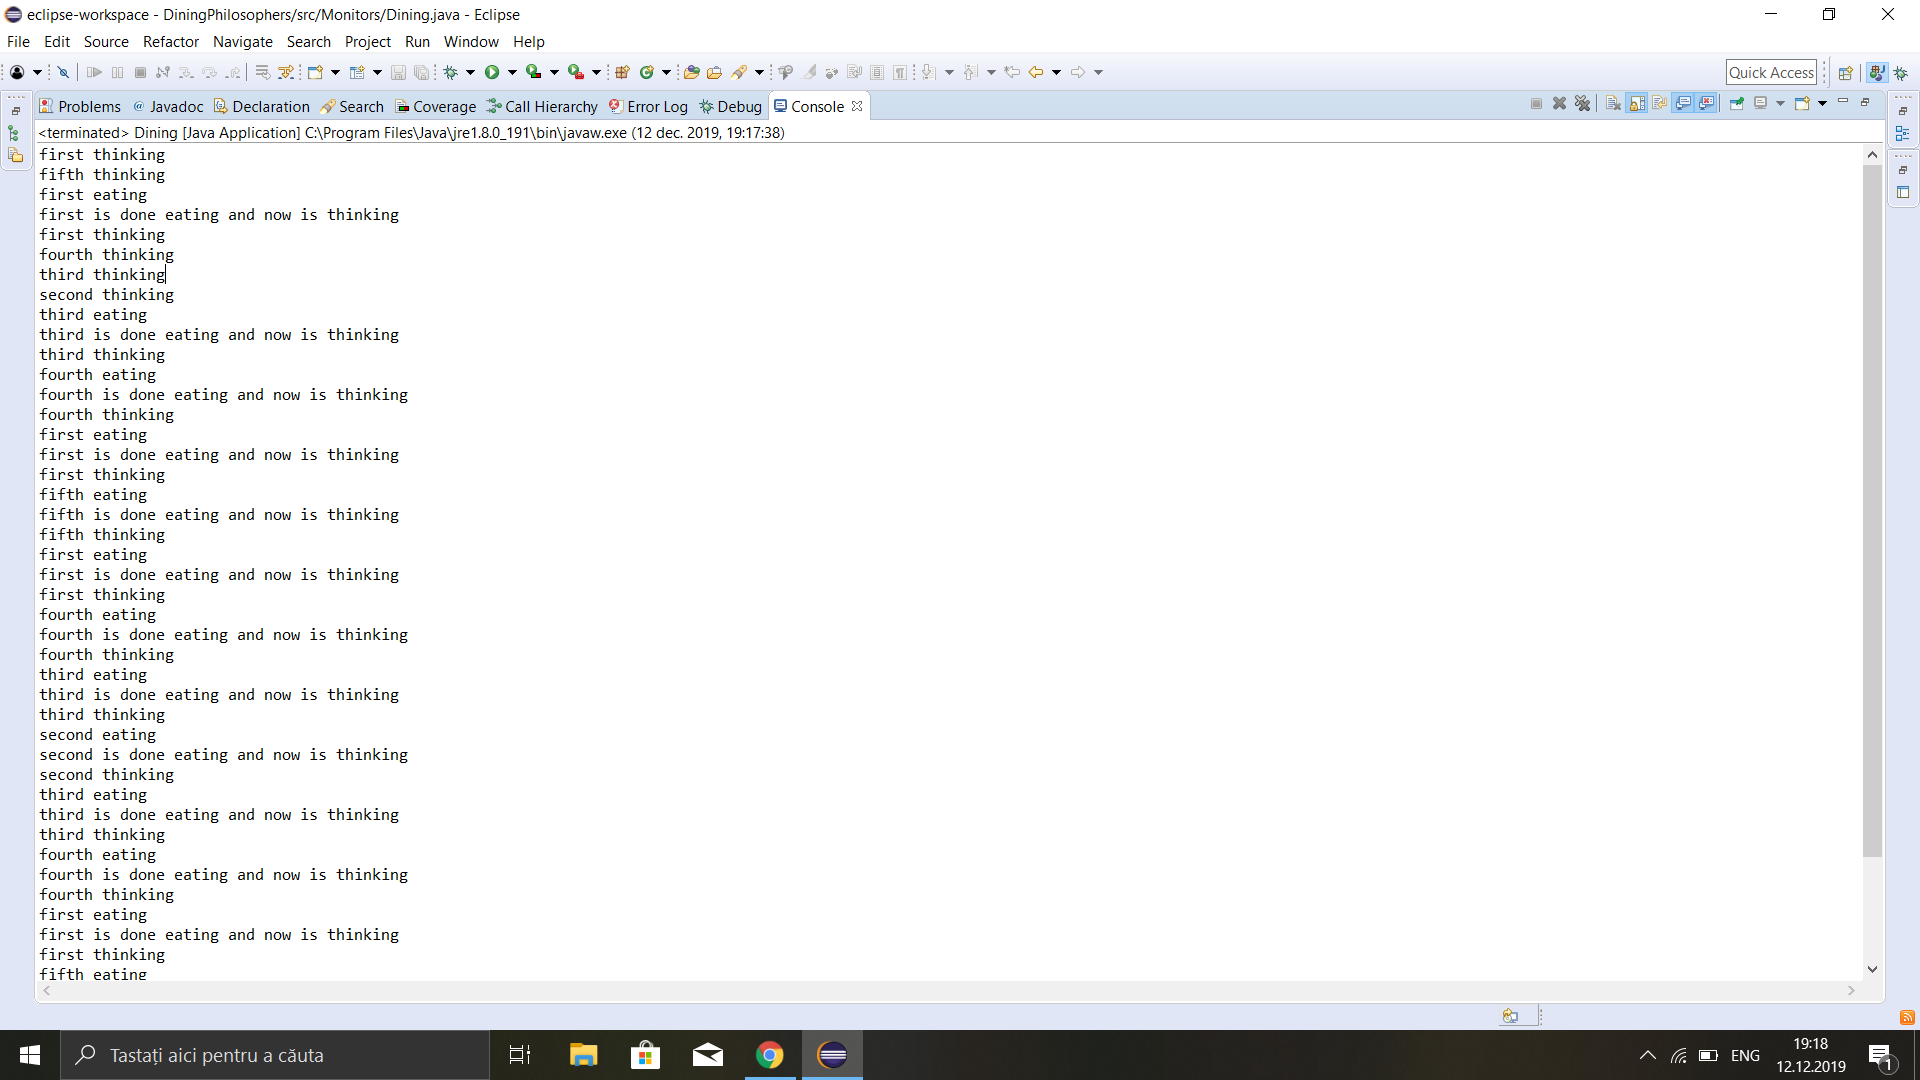
\includegraphics{DPMonitors.png}

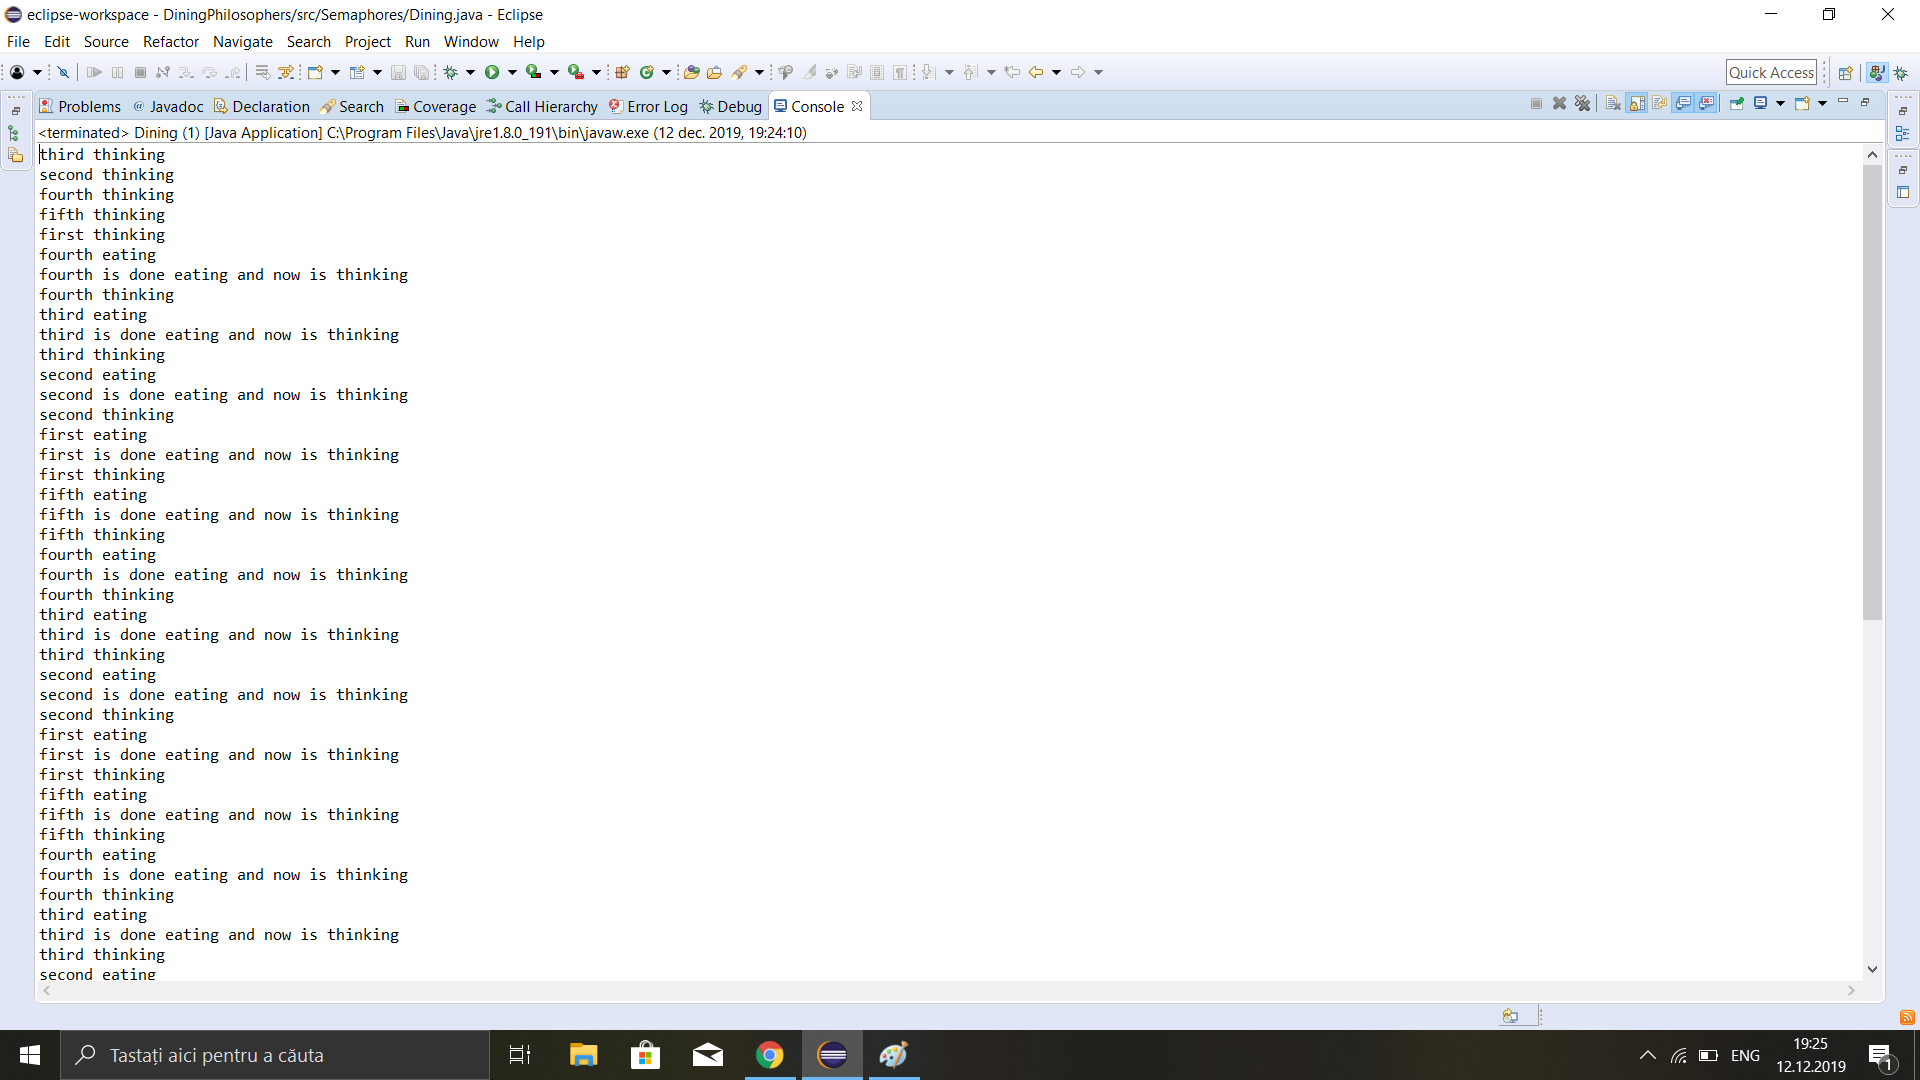
\includegraphics{DPSemaphores.png}

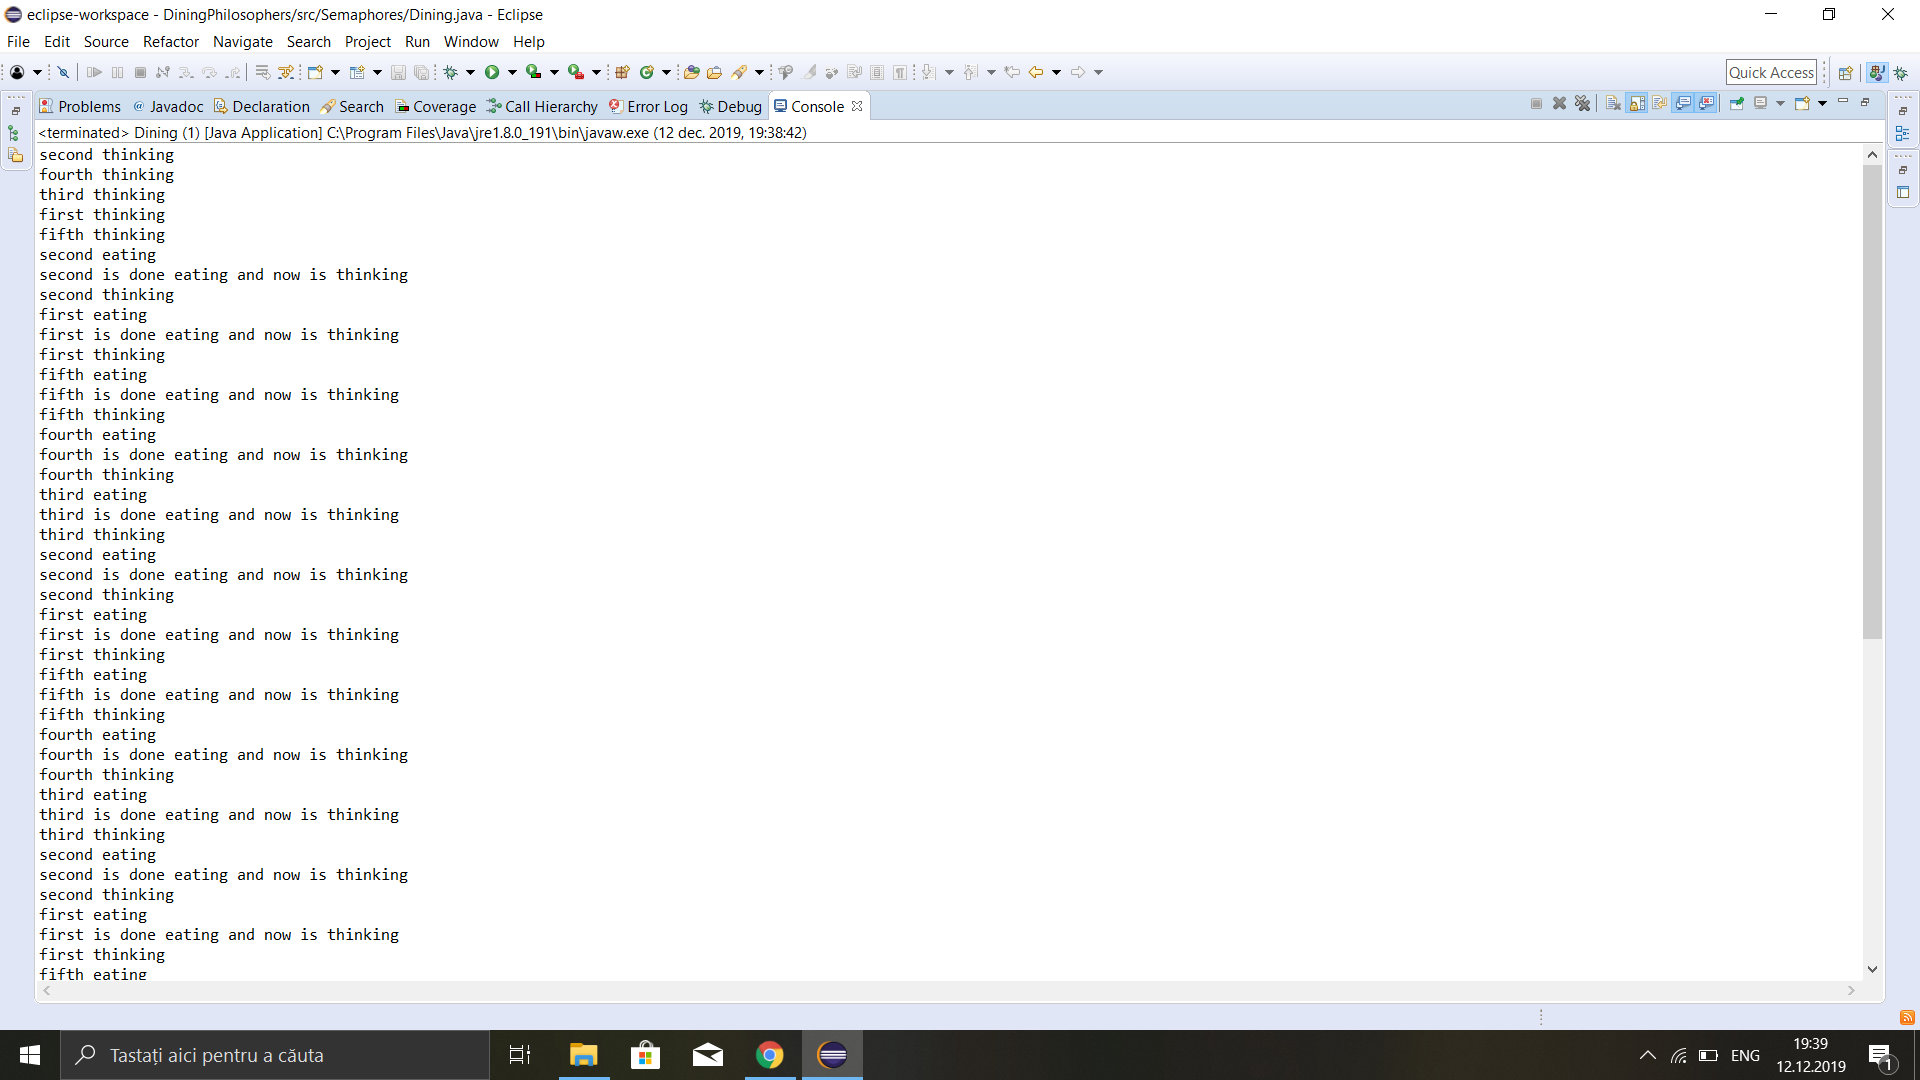
\includegraphics{DPLocks.png}

\section{Results \& Conclusions}
\hspace{0.5 cm}
Am implementat problema cinei filozifilor utilizand 3 metode. Astfel s-a evitat apartitia deadlockul, prin utilizarea diferitelor metode de sincronizare a threadurilor

\end{document}